\documentclass{article}
\usepackage{graphicx} % Required for inserting images
\graphicspath{ {./images/} }
\usepackage{enumitem}
\usepackage[utf8]{inputenc}
\usepackage{bm}
\usepackage{amsmath}
\usepackage{mathtools}% Loads amsmath
\usepackage{amssymb}
\usepackage{multicol}
\usepackage{xcolor}
\usepackage{multirow}
\usepackage{arydshln}

\setlength{\dashlinedash}{4pt}
\setlength{\dashlinegap}{4pt}
\newcommand{\scriptP}{\mathcal{P}}
\allowdisplaybreaks
\usepackage{geometry}
 \geometry{
 a4paper,
 total={170mm,257mm},
 left=17mm,
 top=20mm,
 }
% Footer
\usepackage{fancyhdr}
\newcommand{\E}{\ensuremath{\mathbb{E}}}
\pagestyle{fancy}
\fancyhf{} 
\fancyfoot[L]{MATH3202 A3}
\fancyfoot[C]{Hugo Burton, Lucy Ochre, and Anna Henderson}
\fancyfoot[R]{\thepage}
\renewcommand{\headrulewidth}{0pt} % Remove the line at the top of the page
\renewcommand{\footrulewidth}{0.4pt} % Add a line just above the footer

% cmds
\renewcommand*{\thesection}{\Alph{section}}
\newcommand{\bs}[1]{\boldsymbol{#1}} % remaps \bsboldsymbol to just \bs

\begin{document}
\color{black}
\begin{titlepage}
    \begin{center}
        \vspace*{1cm}
            
        \Huge
        \textbf{MATH3202 Dynamic Programming}
            
        \vspace{0.5cm}
        \Large
        Assignment 3
            
        \vspace{1.5cm}
            
        \textbf{Hugo Burton} (s4698512);\\ \textbf{Lucy Ochre} (s4699043); \&\\ \textbf{Anna Henderson} (s4641893)\\
        \bigskip
        \text{May 2023}
        \vfill
        \text{(Using Hugo's Data)}
        \vfill
        
        %\includegraphics[width=0.4\textwidth]
        \centering{
            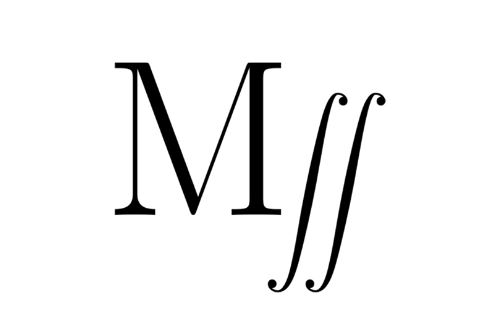
\includegraphics[width=0.25\textwidth]{MSS-logo2}\\
        }
        \vspace{2cm}
        \Large
        UQ Mathematics\\
        The University of Queensland\\
        Australia\\
        Course code: MATH3202
    \end{center}
\end{titlepage}

\section{Report to Boss}
%A general mathematical formulation of the problem, including definitions of sets, data, variables, objective function and constraints. 7 marks • A Python file with the problem modelled for Gurobi. This should be easy to relate back to the formulation. Your boss will attempt to execute this model. 5 marks
\color{black}
\bigskip
As this problem is dynamic programming problem, the structure is as follows

\subsection{Stages}
The stages for this problem are represented by time. Specifically by \textbf{days} over the 14 day period of interest.

\bigskip
\subsection{States}
The only state information that is required is the number of cylinders that are stored overnight for each of the two types (45 kg and 90 kg). This is denoted as $\bs{s_t} = \begin{pmatrix}s_{t,1}\\s_{t,2}\end{pmatrix}$.

\bigskip
\subsection{Data}
\renewcommand\baselinestretch{1.5}
\begin{table}[htb]
    \centering
    \color{black}
    \begin{tabular}{|c:l:c|}
        \hline
        \textbf{Data} & \textbf{Description} & \textbf{Units} \\
        \hline
        $d_{t,1}$ & Regular demand for 45kg cylinders on day $t$ & \# \\ \hdashline
        $h_t$ & High demand for 45kg cylinders on day $t$ & \# \\ \hdashline
        $d_{t,2}$ & Demand for 90kg cylinders on day $t$ & \# \\ \hdashline
        $r_i$ & Revenue for selling cylinder of type $i$ & \$ \\ \hdashline
        $b$ & Base cost of delivery = \$300 & \$ \\ \hdashline
        $c_i$ & Cost of purchasing cylinder type $i$ (excluding base fee) & \$ \\ \hdashline
        $w_i$ & Cylinder $i$'s weight & kg \\ \hdashline
        $M_i$ & Maximum \# of type $i$ cylinders that can be stored overnight & \# \\ \hdashline
        $U$ & Weight limit capacity of truck & kg \\ \hdashline
        $p$ & Probability that demand for type $1$ cylinders is the high demand & $\cdot$ \\ 
        \hline
    \end{tabular}
    \caption{Table of data}
    \label{tab:data}
\end{table}
\renewcommand\baselinestretch{1}

\newpage
The demand for the problem is given in the below table

\renewcommand\baselinestretch{1.5}
\begin{table}[htb]
    \centering
    \color{black}
    \begin{tabular}{|c|c:c:c|}
        \hline
        \textbf{Day} & \textbf{Regular demand 45kg cyls, $d_{t,1}$} & \textbf{High demand 45kg cyls, $h_{t}$} & \textbf{Demand 90kg cyls, $d_{t,2}$} \\
        \hline
        1  & 14 & 17 & 2 \\ \hdashline
        2  & 13 & 17 & 3 \\ \hdashline
        3  & 10 & 15 & 2 \\ \hdashline
        4  & 14 & 21 & 2 \\ \hdashline
        5  & 13 & 21 & 3 \\ \hdashline
        6  & 6  & 14 & 2 \\ \hdashline
        7  & 7  & 16 & 2 \\ \hdashline
        8  & 11 & 17 & 2 \\ \hdashline
        9  & 9  & 15 & 2 \\ \hdashline
        10 & 10 & 19 & 5 \\ \hdashline
        11 & 9  & 12 & 2 \\ \hdashline
        12 & 9  & 16 & 3 \\ \hdashline
        13 & 9  & 13 & 4 \\ \hdashline
        14 & 9  & 13 & 5 \\
        \hline
    \end{tabular}
    \caption{Table of Demand}
    \label{tab:demand}
\end{table}
\renewcommand\baselinestretch{1}
\noindent
The remaining values for this problem were given as
\begin{enumerate}
    \item $r = \begin{pmatrix}\$120 \\ \$230 \end{pmatrix}$
    \item $b = \$ 300$
    \item $c = \begin{pmatrix}\$50 \\ \$80 \end{pmatrix}$
    \item $w = \begin{pmatrix}45 \text{ kg} \\ 90 \text{ kg} \end{pmatrix}$
    \item $M = \begin{pmatrix}30 \\ 2 \end{pmatrix}$
    \item $U = 1000$ kg
    \item $p = 0.4$
\end{enumerate}
\bigskip
\noindent
A few other key points
\begin{itemize}
    \item For the 45 kg cylinders, demand was not required to be met, however, for the 90 kg cylinders, the demand was required to be met.
    \item The maximum number of cylinders that can fit on the truck is limited by the weight limit of the truck. As we know the weights of each type of cylinder, we can perform a dot product of the number of each cylinder purchased with the weights to give the net weight of the cylinders ordered.
    
\end{itemize}

\bigskip
\newpage
\subsection{Actions}

There are three actions to decide each day

\renewcommand\baselinestretch{1.5}
\begin{table}[htb]
    \centering
    \color{black}
    \begin{tabular}{|c:c:c|}
        \hline
        \textbf{Action} & \textbf{Description} & \textbf{Units} \\
        \hline
        $x_{t,i}$ & \# type $i$ cylinders purchased on day $t$ & \# \\ \hdashline
        $y_{t,i}$ & \# type $i$ cylinders sold on day $t$ & \# \\ \hdashline
        $y_{t,2}^*$ & \# 90kg cylinders to swap on day $t$ &  \# \\
        \hline
    \end{tabular}
    \caption{Table of actions}
    \label{tab:actions}
\end{table}
\renewcommand\baselinestretch{1}

Note that since $y_{t,2} = d_{t,2}, \hspace{0.5cm} \forall t \in T$ is a constraint given in the problem, this isn't defined as an action (affects comm 14 and 15 only).

\bigskip
\subsection{Value Function}
\subsubsection{Communication 11}
$$V_t(s_{t,1}) = \underset{\substack{    x_{t,1} \in \{0,...,M_1 - s_{t,1} + y_{t,1}\} \\    y_t \in \{0,...,\min(d_{t,1}, s_{t,1} + x_{t,1})\} }}{\max} \left\{r_1 \cdot y_{t,1} - \min(b \cdot x_{t,1}, b) - c_1\cdot x_{t,1} + V_{t+1}(s_{t,1}-y_{t,1}+x_{t,1}) \right\} $$

with base cases

\begin{align}
    V_t(s_{t,1}) &= 0 & \text{if } s_{t,1} < 0 \hspace{0.125cm} | \hspace{0.125cm} s_{t,1} > M_1 \\
    V_{14}(s_{t,1}) &= 0 & \text{if } t = 14
\end{align}

\subsubsection{Communication 12}

$$V_t(s_{t,1}) = \underset{\substack{ x_{t,1} \in \left\{0,...,\min\left(M_1 - s_{t,1} + y_{t,1},\lfloor\frac{U}{w_1}\rfloor\right)\right\} \\    y_{t,1}t \in \left\{0,...,\min\left(d_{t,1}, s_{t,1} + x_{t,1}\right)\right\} }}{\max} \left\{r_1 \cdot y_{t,1} - \min(b \cdot x_{t,1}, b) - c_1\cdot x_{t,1} + V_{t+1}(s_{t,1}-y_{t,1}+x_{t,1}) \right\} $$

with base cases

\begin{align}
    V_t(s_{t,1}) &= 0 & \text{if } s_{t,1} < 0 \hspace{0.125cm} | \hspace{0.125cm} s_{t,1} > M_1 \\
    V_{14}(s_{t,1}) &= 0 & \text{if } t = 14
\end{align}


\bigskip

\subsubsection{Communication 13}

\begin{align*}
V_t(s_{t,1}) = \underset{\substack{x_{t,1} \in \left\{0,...,\min\left(M_1 - s_{t,1} + y_{t,1},\Big\lfloor \frac{U}{w_1} \Big\rfloor\right)\right\} \\ y_{t,1} \in \left\{0,...,\min\left(h_{t}, s_{t,1} + x_{t,1}\right)\right\} }}{\max} \Biggl\{p \Bigl[C\left(y_{t,1}, x_{t,1}\right) + V_{t+1}(s_{t,1} - y_{t,1}+x_{t,1}) \Bigr] \Biggr. \\
\Biggl.+   (1-p)\Bigl[ C\left(\min(y_{t,1},d_{t,1}), x_{t,1}\right) + V_{t+1}(s_{t,1} - y_{t,1}+x_{t,1})  \Bigr] \Biggr\} 
\end{align*}

with base cases

\begin{align}
    V_t(s_{t,1}) &= 0 & \text{if } s_{t,1} < 0 \hspace{0.125cm} | \hspace{0.125cm} s_{t,1} > M_1 \\
    V_{14}(s_{t,1}) &= 0 & \text{if } t = 14
\end{align}

where

$$C(y_{t,1}, x_{t,1}) = r_1\cdot y_{t,1}- \min\left(x_{t,1} \times b, b\right) - c_1\cdot\begin{pmatrix}x_{t,1}\\x_{t,2}\end{pmatrix}$$

\bigskip
\subsubsection{Communication 14}

% \begin{align*}
%     V_t(s_{t,1},s_{t,2}) = \underset{\substack{x_{t,1} \in \left\{0,...,\min\left(M_1 - s_{t,1} + y_{t,1},\lfloor \frac{U}{w_1\cdot w_2 \cdot x_{t,2}} \rfloor\right)\right\} \\ x_{t,2} \in \left\{0,...,\min\left(M_2 - s_{t,2} + y_{t,2}, \lfloor \frac{U}{w_1\cdot w_2\cdot x_{t,1}} \rfloor\right)\right\} \\ y_{t,1} \in \left\{0,...,\min\left(h_{t}, s_{t,1} + x_{t,1}\right)\right\} \\ y_{t,2} = d_{t,2} \in \left\{0,...,s_{t,2} + x_{t,2}\right\} }}{\max} \biggl\{p \left[C\left(y_{t,1}, y_{t,2}, x_{t,1}, x_{t,2}\right) + V_{t+1}(s_{t,1} - y_{t,1}+x_{t,1}, s_{t,2} - y_{t,2} + x_{t,2}) \right] \biggr. \\
%     \biggl.+ (1-p)\left[ C\left(\min\left(y_{t,1},d_{t,1}\right), y_{t,2}, x_{t,1}, x_{t,2}\right) + V_{t+1}(s_{t,1} - y_{t,1}+x_{t,1}, s_{t,2} - y_{t,2} + x_{t,2})  \right] \biggr\} 
% \end{align*}

% where
% $$C(y_{t,1}, y_{t,2}, x_{t,1}, x_{t,2}) = \bs{r}\cdot\begin{pmatrix}y_{t,1}\\y_{t,2}\end{pmatrix} - \min\left((x_{t,1} + x_{t,2}) \times b, b\right) - \bs{c}\cdot\begin{pmatrix}x_{t,1}\\x_{t,2}\end{pmatrix}$$

\begin{align*}
    V_t(s_{t,1},s_{t,2}) = \underset{\substack{x_{t,1} \in \left\{0,...,\min\left(M_1 - s_{t,1} + y_{t,1},\Big\lfloor \frac{U}{w_1\cdot w_2 \cdot x_{t,2}} \Big\rfloor\right)\right\} \\ x_{t,2} \in \left\{0,...,\min\left(M_2 - s_{t,2} + d_{t,2}, \Big\lfloor \frac{U}{w_1\cdot w_2\cdot x_{t,1}} \Big\rfloor\right)\right\} \\ y_{t,1} \in \left\{0,...,\min\left(h_{t}, s_{t,1} + x_{t,1}\right)\right\} \\ s_{t,2} + x_{t,2} \geq d_{t,2} }}{\max} \Biggl\{p \Bigl[C\left(y_{t,1}, x_{t,1}, x_{t,2}\right) + V_{t+1}(s_{t,1} - y_{t,1}+x_{t,1}, s_{t,2} - d_{t,2} + x_{t,2}) \Bigr] \Biggr. \\
    \Biggl.+ (1-p)\Bigl[ C\left(\min\left(y_{t,1},d_{t,1}\right), x_{t,1}, x_{t,2}\right) + V_{t+1}(s_{t,1} - \min(y_{t,1},d_{t,1})+x_{t,1}, s_{t,2} - d_{t,2} + x_{t,2})  \Bigr] \Biggr\} 
\end{align*}

where
$$C(y_{t,1}, x_{t,1}, x_{t,2}) = \bs{r}\cdot\begin{pmatrix}y_{t,1}\\d_{t,2}\end{pmatrix} - \min\left((x_{t,1} + x_{t,2}) \times b, b\right) - \bs{c}\cdot\begin{pmatrix}x_{t,1}\\x_{t,2}\end{pmatrix}$$


with base cases

\begin{align}
    V_t(s_{t,1},s_{t,2}) &= 0 & \text{if } s_{t,1} < 0 \hspace{0.125cm} | \hspace{0.125cm} s_{t,1} > M_1 \hspace{0.125cm} | \hspace{0.125cm} s_{t,2} < 0 \hspace{0.125cm} | \hspace{0.125cm} s_{t,2} > M_2 \\
    V_{14}(s_{t,1},s_{t,2}) &= 0 & \text{if } t = 14
\end{align}


\bigskip
\subsubsection{Communication 15}

% \begin{align*}
%     V_t(s_{t,1},s_{t,2}) = \underset{\substack{x_{t,1} \in \left\{0,...,\min\left(M_1 - s_{t,1} + y_{t,1},\lfloor \frac{U}{w_1\cdot w_2 \cdot x_{t,2}} \rfloor\right)\right\} \\ x_{t,2} \in \left\{0,...,\min\left(M_2 - s_{t,2} + y_{t,2}, \lfloor \frac{U}{w_1\cdot w_2\cdot x_{t,1}} \rfloor\right)\right\} \\ y_{t,1} \in \left\{0,...,\min\left(h_{t}, s_{t,1} + x_{t,1}\right)\right\} \\ y_{t,2} = d_{t,2} \in \left\{0,...,s_{t,2} + x_{t,2}\right\} }}{\max} \biggl\{p \left[C\left(y_{t,1}, y_{t,2}, x_{t,1}, x_{t,2}\right) + V_{t+1}(s_{t,1} - y_{t,1}+x_{t,1}, s_{t,2} - y_{t,2} + x_{t,2}) \right] \biggr. \\
%     \biggl.+ (1-p)\left[ C\left(\min\left(y_{t,1},d_{t,1}\right), y_{t,2}, x_{t,1}, x_{t,2}\right) + V_{t+1}(s_{t,1} - y_{t,1}+x_{t,1}, s_{t,2} - y_{t,2} + x_{t,2})  \right] \biggr\} 
% \end{align*}

% where
% $$C(y_{t,1}, y_{t,2}, x_{t,1}, x_{t,2}) = \bs{r}\cdot\begin{pmatrix}y_{t,1}\\y_{t,2}\end{pmatrix} - \min\left((x_{t,1} + x_{t,2}) \times b, b\right) - \bs{c}\cdot\begin{pmatrix}x_{t,1}\\x_{t,2}\end{pmatrix}$$

\begin{align*}
    V_t(s_{t,1},s_{t,2}) &= \underset{\substack{x_{t,1} \in \left\{0,...,\min\left(M_1 - s_{t,1} + y_{t,1},\Big\lfloor \frac{U}{w_1\cdot w_2 \cdot x_{t,2}} \Big\rfloor\right)\right\} \\ x_{t,2} \in \left\{0,...,\min\left(M_2 - s_{t,2} + d_{t,2}, \Big\lfloor \frac{U}{w_1\cdot w_2\cdot x_{t,1}} \Big\rfloor\right)\right\} \\ y_{t,1} \in \left\{0,...,\min\left(h_{t}, s_{t,1} + x_{t,1}\right)\right\} \\ y_{t,2}^* \in \left\{0,...,d_{t,2}\right\} \\ s_{t,1}+x_{t,1}-y_{t,1}-2y_{t,2} \in \left\{0,...,M_1\right\} \\ s_{t,2}+x_{t,2}-y_{t,2}+y_{t,2}^* \in \left\{0,...,M_2\right\} \\ y_{t,2}^* \in \left\{0,..., d_{t,2}\}\right\} \\ y_{t,2}+y_{t,2}^* = d_{t,2}}}{\max} \Biggl\{p \Bigl[C\left(y_{t,1}, x_{t,1}, x_{t,2}\right) + \Biggr. \\ \Biggl. &V_{t+1}(s_{t,1} - y_{t,1} - y_{t,2}^* + x_{t,1}, s_{t,2} - y_{t,2}+y_{t,2}^* + x_{t,2}) \Bigr]  \\
    \Biggl.+ &(1-p)\Bigl[ C\left(\min\left(y_{t,1},d_{t,1}\right), x_{t,1}, x_{t,2}\right) \Bigr. \\  \Biggl. &+ V_{t+1}(s_{t,1} - \min(y_{t,1},d_{t,1}) - y_{t,2}^* + x_{t,1}, s_{t,2} - y_{t,2}+y_{t,2}^* + x_{t,2})  \Bigr] - 10y_{t,2}^* \Biggr\} 
\end{align*}

where
$$C(y_{t,1}, x_{t,1}, x_{t,2}) = \bs{r}\cdot\begin{pmatrix}y_{t,1}\\d_{t,2}\end{pmatrix} - \min\left((x_{t,1} + x_{t,2}) \times b, b\right) - \bs{c}\cdot\begin{pmatrix}x_{t,1}\\x_{t,2}\end{pmatrix}$$


with base cases

\begin{align}
    V_t(s_{t,1},s_{t,2}) &= 0 & \text{if } s_{t,1} < 0 \hspace{0.125cm} | \hspace{0.125cm} s_{t,1} > M_1 \hspace{0.125cm} | \hspace{0.125cm} s_{t,2} < 0 \hspace{0.125cm} | \hspace{0.125cm} s_{t,2} > M_2 \\
    V_{14}(s_{t,1},s_{t,2}) &= 0 & \text{if } t = 14
\end{align}

\newpage

\subsection{Solution}
\bigskip
\subsubsection{Communication 11}

The dynamic programming model gave an answer of $\$8810$. Without any weight limit on the truck (like in communications 12 - 15), only 4 deliveries are required on days 1, 4, 7, and 11. For the remaining days, there is enough stock to cover meeting the demand, even though it isn't a requirement that demand is met. \\
\\
The results for this communication are outlined in the following table

\renewcommand\baselinestretch{1.5}
\begin{table}[htb]
    \centering
    \color{black}
    \begin{tabular}{|c:c:c:c:c:c|}
        \hline
        \textbf{Day} & \textbf{Profit} & \textbf{Buy} & \textbf{Weight} & \textbf{Sell} & \textbf{Store} \\
        \hline
        0  & \$8810 & 44 & 1980 & 14 & 30 \\ \hdashline
        1  & \$9630 & 0  & 0    & 13 & 17 \\ \hdashline
        2  & \$8070 & 0  & 0    & 10 & 7  \\ \hdashline
        3  & \$6870 & 37 & 1665 & 14 & 30 \\ \hdashline
        4  & \$7340 & 0  & 0    & 13 & 17 \\ \hdashline
        5  & \$5780 & 0  & 0    & 6  & 11 \\ \hdashline
        6  & \$5060 & 26 & 1170 & 7  & 30 \\ \hdashline
        7  & \$5820 & 0  & 0    & 11 & 19 \\ \hdashline
        8  & \$4500 & 0  & 0    & 9  & 10 \\ \hdashline
        9  & \$3420 & 0  & 0    & 10 & 0  \\ \hdashline
        10 & \$2220 & 36 & 1620 & 9  & 27 \\ \hdashline
        11 & \$3240 & 0  & 0    & 9  & 18 \\ \hdashline
        12 & \$2160 & 0  & 0    & 9  & 9  \\ \hdashline
        13 & \$1080 & 0  & 0    & 9  & 0  \\
        \hline
    \end{tabular}
    \caption{Optimal solution for communication 11}
    \label{tab:comm11}
\end{table}
\renewcommand\baselinestretch{1}
\bigskip
\newpage
\subsubsection{Communication 12}

The dynamic programming model gave an answer of $\$7910$. It is expected that the total profit would reduce because not so many canisters can be ordered at once due to the weight limitation on the truck. This means that more trucks will need to be ordered which results in more base fees being induced, this increasing the price.\\
\\
Note that the difference in costs between communications 12 and 11 is a multiple of the base fee, $\$300$. So $\$8810 - 7910 = \$900 = 3 \cdot \$ 300$.\\
\\
\\The results for this communication are outlined in the following table
\renewcommand\baselinestretch{1.5}
\begin{table}[htb]
    \centering
    \color{black}
    \begin{tabular}{|c:c:c:c:c:c|}
      \hline
      \textbf{Day} & \textbf{Profit} & \textbf{Buy} & \textbf{Weight} & \textbf{Sell} & \textbf{Store} \\
      \hline
      0 & \$7910 & 22 & 990 & 14 & 8 \\ \hdashline
      1 & \$7630 & 22 & 990 & 13 & 17 \\ \hdashline
      2 & \$7470 & 22 & 990 & 10 & 29 \\ \hdashline
      3 & \$7670 & 15 & 675 & 14 & 30 \\ \hdashline
      4 & \$7040 & 0 & 0 & 13 & 17 \\ \hdashline
      5 & \$5480 & 19 & 855 & 6 & 30 \\ \hdashline
      6 & \$6010 & 0 & 0 & 7 & 23 \\ \hdashline
      7 & \$5170 & 0 & 0 & 11 & 12 \\ \hdashline
      8 & \$3850 & 22 & 990 & 9 & 25 \\ \hdashline
      9 & \$4170 & 0 & 0 & 10 & 15 \\ \hdashline
      10 & \$2970 & 21 & 945 & 9 & 27 \\ \hdashline
      11 & \$3240 & 0 & 0 & 9 & 18 \\ \hdashline
      12 & \$2160 & 0 & 0 & 9 & 9 \\ \hdashline
      13 & \$1080 & 0 & 0 & 9 & 0 \\
      \hline
    \end{tabular}
    \caption{Optimal solution for communication 12}
    \label{tab:comm12}
\end{table}
\renewcommand\baselinestretch{1}

\bigskip
\newpage
\subsubsection{Communication 13}
Communication 13 introduced a stochastic nature to the problem where the demand of 45 kg cylinders for any given day was as expected 60\% of the time. But for the other 40\%, the demand was higher, given by $h_t$. As a result, the now total \textit{expected} profit for the two week period was \$9708.08.\\
\\
The truck was expected to make 8 deliveries. This increased from 7 in communication 12 due to the need to account for the higher demand. Note that the actual number of deliveries could potentially be greater as here, 8, is only an expected value.\\
\\
The expected results for this communication are outlined in the following table

\renewcommand\baselinestretch{1.5}
\begin{table}[htb]
    \centering
    \color{black}
    \begin{tabular}{|c|c|c|c|c|c|}
      \hline
      \textbf{Day} & \textbf{Exp Profit} & \textbf{Buy} & \textbf{Weight} & \textbf{Exp Sell} & \textbf{Exp Store} \\
      \hline
      0   & \$ 9708.08 & 22 & 990 & 15 & 6  \\ \hdashline
      1   & \$ 9233.13 & 22 & 990 & 14 & 13 \\ \hdashline
      2   & \$ 8855.65 & 22 & 990 & 12 & 23 \\ \hdashline
      3   & \$ 8816.47 & 0  & 0   & 16 & 6  \\ \hdashline
      4   & \$ 6785.86 & 22 & 990 & 16 & 11 \\ \hdashline
      5   & \$ 6193.77 & 22 & 990 & 9  & 23 \\ \hdashline
      6   & \$ 6437.39 & 0  & 0   & 10 & 12 \\ \hdashline
      7   & \$ 5142.76 & 22 & 990 & 13 & 20 \\ \hdashline
      8   & \$ 4894.93 & 0  & 0   & 11 & 8  \\ \hdashline
      9   & \$ 3481.89 & 22 & 990 & 13 & 16 \\ \hdashline
      10  & \$ 3231.33 & 22 & 990 & 10 & 27 \\ \hdashline
      11  & \$ 3358.88 & 0  & 0   & 11 & 15 \\ \hdashline
      12  & \$ 1876.0  & 0  & 0   & 10 & 4  \\ \hdashline
      13  & \$ 530.0   & 5  & 225 & 9  & 0  \\
      \hline
    \end{tabular}
    \caption{Optimal solution for communication 13}
    \label{tab:comm13}
\end{table}
Note that the Buy - Exp Sell does not equal the Exp Store as this is an expectation rather than an actual selling or storing value
\renewcommand\baselinestretch{1}

\bigskip
\newpage
\subsubsection{Communication 14}

Communication 14 introduced a second type of gas cylinder, weighing 90 kg (double the type 1 cylinders). This raised the total expected profit to \$14346.88 The service centre was required to meet the demand for these heavier cylinders but only had room for 2 of these 90 kg gas cylinders that could be stored overnight. Unlike the 45 kg cylinders, the demand for the 90 kg cylinders was deterministic. Additionally, the 1000 kg weight limit on the delivery truck still applied so that the number of 45kg and 90kg gas cylinders needed to be balanced on the truck in order to maximise profit.\\
\\
As more demand was placed on the same weight limit, the truck was expected to have needed to deliver cylinders on 12 out of the 14 days, where as in communication 13, it was only expected to make 8 deliveries.\\
\\
It is interesting to note that unlike the 45kg cylinders, the 90kg cylinders were rarely stored overnight (in the expected case for each day). This only occur ed on days 7, 8 and 10, each storing 2x 90kg cylinders overnight. This is likely the case due to the restrictive weight limit on the truck. For the preceding days, the demand for 90kg cylinders was 2, 2 and 5, meaning that 4x, 2x, and 7x, 90kg cylinders were required to be ordered. Especially when ordering 7x 90kg cylinders, this eats into the 1000 kg weight limit, meaning that fewer 45kg cylinders can be ordered - thus relying on the maximum 30 of these cylinders that are stocked overnight to supply the next day's demand.\\
\\
The expected results for this communication are outlined in the following table

\renewcommand\baselinestretch{1.5}
\begin{table}[htb]
    \centering
    \color{black}
    \begin{tabular}{|c|c|c:c:c|c:c:c|c|}
        \hline
        \multirow{2}{*}{\centering \textbf{Day}} & \multirow{2}{*}{\centering \textbf{Profit}} & \multicolumn{3}{|c|}{\centering \textbf{45 kg Cylinders}} & \multicolumn{3}{|c|}{\centering \textbf{90 kg Cylinders}} & \multirow{2}{*}{\centering \textbf{Weight}} \\
        \cdashline{3-8}
           &  & \textbf{Buy} & \textbf{Sell} & \textbf{Store for Night} & \textbf{Buy} & \textbf{Sell} & \textbf{Store for Night} &  \\
        \hline
        0  & \$ 14346.88 & 18  & 15 & 2  & 2 & 2 & 0 & 990 \\ \hdashline
        1  & \$ 13370.78 & 16  & 14 & 3  & 3 & 3 & 0 & 990 \\ \hdashline
        2  & \$ 12246.4  & 18  & 12 & 9  & 2 & 2 & 0 & 990 \\ \hdashline
        3  & \$ 11710.23 & 18  & 16 & 10 & 2 & 2 & 0 & 990 \\ \hdashline
        4  & \$ 10581.69 & 16  & 16 & 9  & 3 & 3 & 0 & 990 \\ \hdashline
        5  & \$ 9242.21  & 18  & 9  & 17 & 2 & 2 & 0 & 990 \\ \hdashline
        6  & \$ 8985.44  & 14  & 10 & 20 & 4 & 2 & 2 & 990 \\ \hdashline
        7  & \$ 8551.54  & 18  & 13 & 24 & 2 & 2 & 2 & 990 \\ \hdashline
        8  & \$ 7780.0   & 0   & 11 & 12 & 0 & 2 & 0 & 0   \\ \hdashline
        9  & \$ 5960.4   & 8   & 13 & 6  & 7 & 5 & 2 & 990 \\ \hdashline
        10 & \$ 4278.0   & 0   & 6  & 0  & 0 & 2 & 0 & 0   \\ \hdashline
        11 & \$ 3098.0   & 16  & 11 & 4  & 3 & 3 & 0 & 990 \\ \hdashline
        12 & \$ 2322.0   & 14  & 10 & 7  & 4 & 4 & 0 & 990 \\ \hdashline
        13 & \$ 1430.0   & 2   & 9  & 0  & 5 & 5 & 0 & 540 \\
        \hline
    \end{tabular}
    \caption{Optimal solution for communication 14}
    \label{tab:comm14}
\end{table}
\renewcommand\baselinestretch{1}

\bigskip
\newpage
\subsubsection{Communication 15}


Communication 15 allowed 90kg cylinders to be swapped for 2x 45kg cylinders. Even though this costs an extra \$10 per swap, it has the potential to save a delivery, thus increasing profit. The total expected optimal profit was further increased to \$14609.13 which is \$262.15 higher than communication 14.\\
\\
The reasons for this increased are discussed in the presentation - part B.


\bigskip
\color{black}
\end{document}